\chapter{Tensorflow API}
\section{tf.clip\_by\_value}
clip\_by\_value(t,clip\_value\_min,clip\_value\_max,name=None):剪切值为最大值和最小值,给定一个tensor t,操作返回一个和t同样类型,同样大小的值到clip\_value\_min,和clip\_value\_max.任何值小鱼clip\_value\_min被设置为clip\_value\_min,任何大于clip\_value\_max的值被设置为clip\_value\_max。
参数:
\begin{itemize}
	\item t:一个tensor
	\item clip\_value\_min:一个0维Tensor或者和t相同形状的tensor,取代的最小值
	\item clip\_value\_max:一个0维Tensor或者和t有相同形状的Tensor,取代的大值
	\item name:操作的名字
	\item[Returns]:一个取代后的tensor。
	\item[Raises]:如果剪切的tensor将触发数组的广播操作将安徽比输入更大的返回tensor。
\end{itemize}
\section{tf.app.flags}
\subsection{DEFINE\_boolean}
DEFINE\_boolean(flag\_name,default\_value,docstring):定义一个'boolean'类型的flag。
\begin{itemize}
\item flag\_name:flag的名字,是一个字符串。
\item default\_value:flag应被被看作一个boolean的默认值。
\item docstring:用flag的一个帮助信息。
\end{itemize}
\subsection{DEFINE\_boolean}:定义一个'boolean'类型的flag。
\begin{itemize}
\item flag\_name:flag的名字,是一个字符串。
\item flag\_default\_value:默认的boolean类型的值。
\item docstring:用flag的一个有用的帮助信息。
\end{itemize}
\subsection{DEFINE\_float}:定义一个浮点数类型的flag。
\begin{itemize}
\item flag\_name:作为flag的名字,应该是字符串。
\item default\_value:flag的默认值,应该是浮点数。
\item docstring:用flag的一个有用的帮助信息。
\end{itemize}
\subsection{DEFINE\_integer}:定义一个整数的flag。
\begin{itemize}
\item flag\_name:flag的名字,应该是字符串。
\item default\_value:flag的默认值,应该是一个整数。
\item docstring:用flag的一个有用的帮助信息。
\end{itemize}
\subsection{DEFINE\_string}:定义一个字符串的flag。
\begin{itemize}
\item flag的名字,应该是字符串。
\item default\_value:flag的默认值,应该是字符串。
\item docstring:用flag的一个有用的帮助信息。
\end{itemize}
\subsection{tf.gather}
\begin{python}
gather(
    params,
    indices,
    validate_indices=None,
    name=None,
    axis=0
	)
\end{python}
根据indices从params和axis轴获取slices。
indices必须是任何维度(通常是0维或者一维)的一个整数tensor生成输出tensor的形状params.shape[:axis]+indices.shape+params.shape[axis+1:],这里
\begin{python}
# Scalar indices (output is rank(params) - 1).
output[a_0, ..., a_n, b_0, ..., b_n] =
params[a_0, ..., a_n, indices, b_0, ..., b_n]
# Vector indices (output is rank(params)).
output[a_0, ..., a_n, i, b_0, ..., b_n] =
params[a_0, ..., a_n, indices[i], b_0, ..., b_n]
# Higher rank indices (output is rank(params) + rank(indices) - 1).
output[a_0, ..., a_n, i, ..., j, b_0, ... b_n] =
params[a_0, ..., a_n, indices[i, ..., j], b_0, ..., b_n]
\end{python}
\begin{figure}[H]
	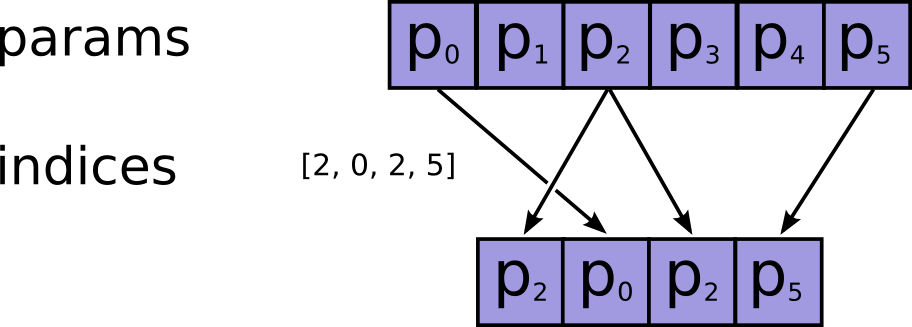
\includegraphics[scale=0.5]{Gather.png}
\end{figure}
参数:
\begin{itemize}
	\item params:一个Tensor,从它那里收集值,rank必须是axis+1
	\item indices:一个tensor。必须是int32,int64.索引tensor,必须是在[0,params.shape[axis])
	\item axis:一个Tensor,必须是下面的数据类型:int32,int64.params的轴,从params中获得收集索引,默认是第一维,支持负索引。
	\item name:操作的名字
	\item{返回}:一个tensor,和params有相同的数据类型,通过给定indeces从params收集,形状为[params.shape[:axis]+indices.shape+params.shape[axis+1:]
\end{itemize}
例子:
\begin{python}
import tensorflow as tf
a = tf.constant([[1,2,3,4],[5,6,7,8],[9,10,11,12],[13,14,15,16]])
b = tf.constant([1,0,2])
g = tf.gather(a,b)
with tf.Session() as sess:
    print(sess.run(g))#获取第一轴[1,0,2]行的数据
\end{python}
输出:
\begin{python}
[[ 5  6  7  8]
 [ 1  2  3  4]
 [ 9 10 11 12]]
\end{python}
\subsection{tf.placeholder}
\begin{python}
placeholder(
    dtype,
    shape=None,
    name=None
)
\end{python}
为placeholder输入需要被插入的tensor。
如果这个tensor被计算将产生错误。他的值必须通过feed\_dict选项在Session.run(),Tensor.eval()或者是Operation.eval()输入。
\begin{python}
x = tf.placeholder(tf.float32, shape=(1024, 1024))
y = tf.matmul(x, x)
with tf.Session() as sess:
    print(sess.run(y))  # ERROR: will fail because x was not fed.
    rand_array = np.random.rand(1024, 1024)
    print(sess.run(y, feed_dict={x: rand_array}))  # Will succeed.
\end{python}
参数:
\begin{itemize}
\item dtype:被输入的tensor元素的数据类型。
\item shape:被fed的tensor的形状,如果形状没有被指定,你可以输入任何形状的tensor。
\item:操作的名字
\item{Return} 一个可能被用作输入数据处理的Tensor,值不能被直接计算。
\end{itemize}
\subsection{tf.squeeze}
tf.squeeze(input,axis=None,name=None,squeeze\_dims=None)
说明:从指定的Tensor中移除1维度。
\begin{itemize}
\item input:tensor,输入Tensor。
\item axis:列表,指定需要移除的位置的列表,默认为空列表[],索引从0开始squeeze不为1的索引会报错。
\item name:操作的名字
\item squeeze\_dims:否决当前轴的参数。
\item 返回一个Tensor,形状和input相同,包含和input相同的数据,但是不包含有1的元素。
\item 异常:squeeze\_dims和axis同时指定时会有ValueError。
\end{itemize}
\# 't' is a tensor of shape [1, 2, 1, 3, 1, 1]\newline
shape(squeeze(t)) ==> [2, 3]\newline
\# 't' is a tensor of shape [1, 2, 1, 3, 1, 1]\newline
shape(squeeze(t, [2, 4])) ==> [1, 2, 3, 1]\newline
\subsection{tf.metrics}
accuracy(labels,predictions,weights=none,metrics\_collections,updates\_collections=none,name=none)
\begin{itemize}
	\item labels:tensor,和predictions的形状相同,代表真实值。
	\item predictions:tensor,代表预测值。
	\item weights:tensor,rank可以为0或者labels的rank,必须能和label广播(所有的维度必须是1,或者和labels维度相同)
	\item metrics\_collection:accuracy应该被增加的一个collectiobn列表选项。
	\item update\_collections:update\_op应该添加的选项列表。
	\item name:variable\_scope名字选项。
	\item accuracy:返回值tensor,代表精度,总共预测对的和总数的商。
	\item update\_op:返回值适当增加total和count变量和accuracy匹配。
	\item valueerror:异常如果predictions和labels有不同的形状,或者weight不是none它的形状不合prediction匹配,或者metrics\_collections会哦这updates\_collections不是一个list或者tuple。
\end{itemize}
\subsection{tf.split}
split(value,num\_or\_size\_splits,axis=0,num=None,name='split'):分割一个Tensor,如果num\_or\_size\_split是一个整数类型,num\_split然后沿着axis分割value为num\_split更小的tensors。要求num\_split均匀分割为value.shape[axis]。如果num\_or\_size\_splits不是一个整数类型,它被将定位一个Tensorsize\_splits,然后分割值为len(size\_splits)段,第i个形状有相同的大小作为value除了沿着维度axis,这里的size是size\_splits[i]。
\begin{lstlisting}[language=Python]
#value是一个形状为[5,30]的tensor
#分割沿着1轴分割'value'为3个tensor,形状为【4,15,11】
split0,split1,split2 = tf.split(value,[4,15,11],1)
tf.shape(split0) ==>[5,4]
tf.shape(split1) ==>[5,15]
tf.shape(split2) ==>[5,11]
#沿着1轴分割‘value’为三个tensor
split0,split1,split2 = tf.split(value,num_or_size_split=3,axis=1)
tf.shape(split0) ==>[5,10]
\end{lstlisting}
参数:
\begin{itemize}
	\item value:要分割的Tensor
	\item num\_or\_size\_splits:是一个0维整数Tensor,表示沿着split\_dim或者包含每个分割长度的1维整数tensor分割多少份。如果是标量将被均匀分割为value.shape[axis]。否者沿着分割维度求和必须和value匹配。
	\item axis:0维 int32 tensor,沿着分割的维度,必须在[-rank(value),rank(value)],默认为0。
	\item num:选项,不能推断出时用于指定size\_split输出数
	\item name:操作的名字
	\item [Returns]:如果num\_or\_size\_split是一个标量返回num\_or\_size\_split是一个一维Tensor返回value分割的num\_or\_size\_splits.get\_shape[0] Tensor对象
	\item [Raises]:如果num不被指定也不能被推断出。将产生ValueError
\end{itemize}
\subsection{tf.stack}
stack(values,axis=0,name='stack'):stack一个n维tensor为n+1维tensor。
给定一个长度为N的形状为(A,B,C)的tensor,如果axis==0输出tensor的形状为(N,A,B,C),如果axis==1,输出tensor的形状为(A,N,B,C)
\# 'x' is [1,4]\newline
\# 'y' is [3,6]\newline
\# 'z' is [3,6]\newline
stack([x,y,z])==>[[1,4],[2,5],[3,6]]\newline
stack(x,y,z,axis=1)==>[[1,2,3],[4,5,6]]\newline
tf.stack([x,y,z]) = np.asarray([x,y,z])\newline
输出参数:
\begin{itemize}
	\item 一个Tensor列表。
	\item 整数,默认为0,支持负坐标。
	\item 操作的名字。
	\item[\S] 一个stack的Tensor。
	\item[\S] ValueError:如果axis超过[-(R+1),R+1)
\end{itemize}
\textsl{Example}
\begin{python}
import tensorflow as tf
x = tf.constant([1,4])
y = tf.constant([2,5])
z = tf.constant([3,6])
r1 = tf.stack([x,y,z])
r2 = tf.stack([x,y,z],axis=1)
with tf.Session() as sess:
    print(sess.run(r1).shape)
    print(sess.run(r2).shape)
\end{python}
\subsection{tf.reshape}
tf.reshape(tensor,shape,name=None)
\begin{itemize}
	\item Tensor:一个Tensor。
	\item shape:一个列表,数值类型为int32或者时int64
	\item name:操作的名字。
	\item[S] 指定形状的Tensor。
\end{itemize}
\begin{python}
import tensorflow as tf
a = tf.linspace(0.,9.,10)
b = tf.reshape(a,[2,5])
with tf.Session() as sess:
    a = sess.run(a)
    b = sess.run(b)
print(a.shape)
print(b.shape)
\end{python}
\subsection{tf.random\_crop}
\begin{python}
random_crop(
    value,
    size,
    seed=None,
    name=None
)
\end{python}
从value tensor随机剪裁一块指定size的tensor,要求value。shape大于参数size的值。如果一维不剪切需要传递完整的size,例如RGB图像可以用size = [crop\_height,crop\_width,3]剪切。

输入参数:
\begin{itemize}
\item value:需要被剪切的tensor
\item size:和value有相同rank的一维tensor。
\item seed:Python整数,用于创建一个随机种子。
\item name:操作的名字。
\item[Retuen] 一个剪切的和value有相同的rank,形状为size的tensor。
\end{itemize}
\subsection{tf.random\_gamma}
\begin{python}
random_gamma(
    shape,
    alpha,
    beta=None,
    dtype=tf.float32,
    seed=None,
    name=None
)
\end{python}
从指定\href{https://zh.wikipedia.org/wiki/伽玛分布}{Gamma分布}中获得shape样本,alpha是形状参数,beta是反向放大参数。

输入参数:
\begin{itemize}
\item shape:一个一维整数Tensor或者Python数组,指定alpha,beta参数的输出采样数据。
\item alpha:一个tensor或者python值或者N维dtype数据类型。alpha提供形状参数,必须和beta广播。
\item beta:一个tensor或python值或者dtype类型的n维数组。默认为1.beta提供gamma分布的反向放大参数。必须和alpha广播。
\item dtype:alpha,beta,output的输出:float16,float32或者float64。
\item seed:一个Python整数,用于创建随机种子。
\item name:操作的选项。
\item[Returns]:
samples:数据类型为dtype的一个形状为tf.concat(shape,tf.shape(alpha+beta))的tensor。
\end{itemize}
例子:
\begin{python}
samples = tf.random_gamma([10],[0.5,1.5])#形状为10,alpha为0.5,1.5,采样输出形状为[10,2]
samples = tf.random_gamma([7, 5], [0.5, 1.5]) # 采样输出形状为[7, 5, 2], where each slice [:, :, 0] and [:, :, 1] # 代表从两个分布采样的$7\items5$。
samples = tf.random_gamma([30], [[1.],[3.],[5.]], beta=[[3., 4.]]) #采样输出形状[30, 3, 2], 每$2\times2$(广播运算)30个采样点
\end{python}
\subsection{tf.random\_normal}
\begin{python}
random_normal(
    shape,
    mean=0.0,
    stddev=1.0,
    dtype=tf.float32,
    seed=None,
    name=None
)
\end{python}
输出正态分布随机值。

输入参数:
\begin{itemize}
\item shape:一个一维整数tensor或者Python数组。表示输出tensor的形状。
\item mean:一个0维tensor和dtype的Python值,正态分布的均值。
\item stddev:一个0维tensor和dtype的Python值,正态分布的标准差。
\item stype:输出数据类型。
\item seed:一个整数,用于创建一个随机数种子。
\item name:操作的名字。
\item[Returns] 制订形状的正态分布值。
\end{itemize}
\subsection{\textbf{tf.random\_normal\_initializer}}
继承于\href{https://www.tensorflow.org/api_docs/python/tf/contrib/keras/initializers/Initializer}{Initializer}
别名:
\begin{itemize}
\item Class tf.contrib.keras.initializers.RandomNormal
\item Class tf.random\_normal\_initializer
\end{itemize}
输入参数:
\begin{itemize}
\item mean:一个python标量或者标量tensor。生成随机值的均值。
\item stddev:一个python标量或者标量tensor。标生成随机值的标准差。
\item seed:python整数,用于创建随机种子。
\item dtypes:数据类型,仅仅支持浮点数类型。
\end{itemize}
方法:
\begin{itemize}
\item \_\_init\_\_
\begin{python}
__init__(
    mean=0.0,
    stddev=1.0,
    seed=None,
    dtype=tf.float32
)
\end{python}
\item \_\_call\_\_
\begin{python}
__call__(
    shape,
    dtype=None,
    partition_info=None
)
\end{python}
\item from\_config:从配置字典实例化initilizer。
\begin{python}
from_config(
    cls,
    config
)
\end{python}
例如:
\begin{python}
initializer = RandomUniform(-1, 1)
config = initializer.get_config()
initializer = RandomUniform.from_config(config)
\end{python}
\item get\_config()
\end{itemize}
\subsection{tf.random\_possion}
\begin{python}
random_poisson(
    lam,
    shape,
    dtype=tf.float32,
    seed=None,
    name=None
)
\end{python}
从Poisson分布中获取制定形状的样本,lam是描述分布的参数。

输入参数:
\begin{itemize}
\item lam:一个Tensor或者Python值或者dtype指定的N维数组。lam是Poisson分布的参数。
\item shape:yuige一维整数tensor或者python数组,输出每个rate指定的参数的形状。
\item dtype:lam和输出的数据类型:float16,float32,float64.
\item seed:Python整数,用于创建一个分布的随机种子。
\item name:操作的名字。
\item[Returns]:形状为tf.concat(shape,tf,shape(lam))的tensor(值的数据类型如dtype指定)。
\end{itemize}
例子:
\begin{python}
samples = tf.random_poisson([0.5, 1.5], [10]) # 采样输出形状为[10, 2],切片输出 [:, 0] and [:, 1] 代表不同分布的数据

samples = tf.random_poisson([12.2, 3.3], [7, 5]) # 采样输出形状[7, 5, 2], chide切片[:, :, 0]和[:, :, 1]代表 $7\times5$从两个分布的采样输出。
\end{python}
\subsection{random\_shuffle}
\begin{python}
random_shuffle(
    value,
    seed=None,
    name=None
)
\end{python}
沿着tensor的一维随机打乱数据。像value[j]映射一个tensor到一个数出output[i]。例如
\begin{python}
[[1, 2],       [[5, 6],
 [3, 4],  ==>   [1, 2],
 [5, 6]]        [3, 4]]
\end{python}
输入参数:
\begin{itemize}
\item value:一个应该被打乱的值。
\item seed:一个python正数用于创建随机数种子。
\item name:操作的名字。
\item[Returns] 一个指定类型的值和形状,沿着某一维读被打乱的tensor。
\end{itemize}
\subsection{tf.random\_uniform}
\begin{python}
random_uniform(
    shape,
    minval=0,
    maxval=None,
    dtype=tf.float32,
    seed=None,
    name=None
)
\end{python}
输出均匀分布的随机值,生成的值的范围在[minival,maxval),下界minval包含在范围内,上界不再。对于浮点数默认范围是[0,1)。至少maxval必须被明确指定。在整数情况下,会有一些轻微的偏移,除非maxval-minval是2的次幂。偏移是maxval-minval
比较小的值相对于输出范围(2**32,2**64)很小。

输入参数:
\begin{itemize}
\item shape:一维整数tensor或者Python数组,和数出tensor的形状相同。
\item minval:0维tensor或者dtype指定的python值,生成随机数的下界,默认为0,。
\item maxval:0维tensor或者dtype指定的python值。生成随机数的上界,dtype是浮点数时,默认为1。
\item dtype:输出的类型:'float16,float32,float64,int32,int64'。
\item seed:一个Python整数。用于创建分布的随机数种子。
\item 操作的名字。
\item [Return] 返回指定形状的均匀分布值。
\item [Raise] ValueError:如果dtype是整数并且maxval没有被指定。
\end{itemize}
\subsection{\textbf{tf.random\_uniform\_initializer}}
一个继承自Initilizer的类。

别名:
\begin{itemize}
\item tf.contrib.keras.initializers.RandomUniform
\item tf.random\_uniform\_initializer
\end{itemize}
生成均匀分布tensor的initializer。

输入参数:
\begin{itemize}
\item minval:0维tensor或者dtype指定的python值,生成随机数的下界,默认为0,。
\item maxval:0维tensor或者dtype指定的python值。生成随机数的上界,dtype是浮点数时,默认为1。
\item seed:一个Python整数。用于创建分布的随机数种子。
\item dtype:输出的类型:'float16,float32,float64,int32,int64'。
\end{itemize}
方法:
\begin{itemize}
\item \begin{python}__init__(
    minval=0,
    maxval=None,
    seed=None,
    dtype=tf.float32
)\end{python}
\item \_\_call\_\_
\begin{python}
__call__(
    shape,
    dtype=None,
    partition_info=None
)
\end{python}
\item from\_config
\begin{python}
from_config

from_config(
    cls,
    config
)
\end{python}
\item get\_config
\end{itemize}
\subsection{tf.transpose}
tf.transpose(a,perm=none,name='transpose'):根据perm改变a的维度,返回一个tensor,它的维度i和perm[i]对应,如果perm没有给定,它被设置为(n-1,\ldots,0),z这是n是输入tensor的rank,输入是2维tensor是执行常规的转置操作:
\begin{lstlisting}[language=Python]
# 'x' is[[1 2 3],[4 5 6]]
tf.transpose(x)==>[[1 4]
		   [2 5]
		   [3 6]]
#等价于
tf,transpose(x,[1,0])==>[[1 4]
			 [2 5]
			 [3 6]]
# perm对于n为tensor很有用,n>2
# x  [[[1,2,3]
#       [4,5,6]]
#       [[7 8 9]
#       [10,11,12]]]
tf.transpose(x,perm=[0,2,1])==>[[[1 4]
				[2 5]
				[3,6]]

				[[7 10]
				[8 11]
				[9 12]]]
\end{lstlisting}
参数:
\begin{itemize}
	\item a:一个Tensor
	\item perm:一个a的维度的乱序
	\item name:操作的名字
	\item[Return] 一个转置后的Tensor
\end{itemize}
\subsection{tf.one\_hot}
\begin{python}
ne_hot(
    indices,
    depth,
    on_value=None,
    off_value=None,
    axis=None,
    dtype=None,
    name=None
)
\end{python}
返回一个One-hot tensor。
indices表示的下表的值为on\_value,所有其它值为off\_value。

如果on\_value不提供,默认为dtype下的1。off\_value不提供,默认值为0,如果输入Incices rank是N,输出rank将是N+1。新的axis将在axis创建。,如果indices是一个标量,输出形状将是一个depth长度的向量,如果indices是亿个长度为features向量输出形状将为:
\begin{python}
feature x depth ifn axis == -1
depth x features if axis == 0
\end{python}
如果indices是一个矩阵,形状为[batch,features],输出形状将为:
\begin{python}
 batch x features x depth if axis == -1
  batch x depth x features if axis == 1
  depth x batch x features if axis == 0
\end{python}
如果dtype没有被提供,他将假设on\_value或off\_value的数据类型,如果一个或者倍多的值呗传递,,如果没有on\_value,off\_value,或者dtype被提供,dtype将默认tf.float32。
例子:

假设:
\begin{python}
indices = [0, 2, -1, 1]
  depth = 3
  on_value = 5.0
  off_value = 0.0
  axis = -1
\end{python}
输出形状为[$4\times3$]
输出:
\begin{python}
output =
  [5.0 0.0 0.0]  // one_hot(0)
  [0.0 0.0 5.0]  // one_hot(2)
  [0.0 0.0 0.0]  // one_hot(-1)
  [0.0 5.0 0.0]  // one_hot(1)
\end{python}
假设:
\begin{python}
 indices = [[0, 2], [1, -1]]
  depth = 3
  on_value = 1.0
  off_value = 0.0
  axis = -1

\end{python}
输出
\begin{python}
output =
  [
    [1.0, 0.0, 0.0]  // one_hot(0)
    [0.0, 0.0, 1.0]  // one_hot(2)
  ][
    [0.0, 1.0, 0.0]  // one_hot(1)
    [0.0, 0.0, 0.0]  // one_hot(-1)
  ]
\end{python}
用默认on\_value和off\_value:
\begin{python}
indices = [0, 1, 2]
  depth = 3
\end{python}
输出
\begin{python}
  output =
  [[1., 0., 0.],
   [0., 1., 0.],
   [0., 0., 1.]]
\end{python}
参数:
\begin{itemize}
\item indices:一个索引的Tensor。
\item depth:一个定义one hot维度的深度的标量。
\item on\_vlaue:制定Indices[j]=i(填入i),默认为1。
\item off\_value:一个标量当Indices[j]!=i(默认为0)。
\item axis:填入的轴,默认为-1。
\item dtype:输出tensor的数据类型。
\item [Returns]:one-hot tensor。
\item [Raise]
\begin{itemize}
\item TypeError:如果dtype和on\_value,off\_value数据类型不一样。
\item TypeError:如果on\_value和off\_value不合另一个匹配。
\end{itemize}
\end{itemize}
\subsection{tf.unstack}
\begin{python}
unstack(
    value,
    num=None,
    axis=0,
    name='unstack'
)
\end{python}
unstack rank-R为rank-(R-1)的tensor。通过chipping沿着axis从value unstack num tensor。如果num不被指定(默认)它从value的形状推算。如果value.shape[axis]不知道,ValueError异常。
例如一个tensor的形状为(A,B<C<D);
如果 axis ==0输出第i维的切片value[i,:,:,:],output的输出每个tensor形状为(B,C,D).(注意沿着维度unstack)
如果axis == 1然后输出第i个tensor在切片的值[:,i,:,:]和每个output的每个输出将有形状(A,C,D)。
tf.ustack(x,n)=list(x)

参数:
\begin{itemize}
\item value:rank R>0的Tensor能被unstack。
\item num 一个整数。axis的长度,如果为None将自动推断。
\item axis:一个整数。ustack沿着的轴。默认是第一维,支持负的索引。
\item name:操作的名字。
\item[Returns] 从value unstack的Tensor列表。
\item[Raises]:
\begin{itemize}
\item ValueError:如果num没有被指定且不能推断出。
\item ValueError:如果axis超过[-R,R)。
\end{itemize}
\end{itemize}
\subsection{tf.contrib.rnn}
\subsubsection{AttentionCellWrapper}
继承自RNNCell,是一个基本的attention cell包装器。\newline
\begin{tabular}{|c|c|}
	graph&\_\_init\_\_\\
	losses&\_\_call\_\_\\
	non\_trainable\_variables&\_\_deepcopy\_\_\\
	non\_trainable\_weights&add\_loss\\
	output\_size&add\_update\\
	scope\_size&add\_variable\\
	state\_size&apply\\
	trainable\_variable&build\\
	trainable\_weights&call\\
	updates&get\_losses\_for\\
	vaiables&get\_updates\_for\\
	weights&zero\_state\\
\end{tabular}
